\documentclass{svmult}
\usepackage{graphicx}
\begin{document}
\title{ : A Tool for Consistency and Satisfiability analysis of 
		Assertion Specifications}

\maketitle
\thispagestyle{empty}

\abstract
{
Software Verification has become a must necessary step of Software engineering.
For performing software verification we need to have a well written requirement 
Specification. Generally requirements are written in Natural Language processing
which can be ambiguous or may have contradictory requirements. If a code is verified 
against this erroneous specification it cannot result to a correct software output.
In this paper we want to present a tool ToYicesTranslator  that can check if the 
requirements are inconsisten or unsatisfiable.This tool consists of 3 parts, First 
our input file is given to a parser,it will generate a symb0l table and a syatax tree.
Now using this symbol table and sysntax tree ToYicesTranslator will generate a file 
which is compatible with Yices.Yices is tool for checking satisfiability of the given 
expression.If Yices gives SAT as result then the given specifications is satisfiable 
and consistent.
}


\section{Introduction}

In recent times, most leading chip design companies are seriously attempting 
to induct assertion-based verification techniques in the pre-silicon 
validation flows. The advantages of specifying the key features of the design 
intent in terms of formal properties are increasingly being 
acknowledged and accepted by validation engineers and design managers. 
Property suites for standard interfaces, such as PCI Express, ARM AMBA, and 
USB are in considerable demand. System Verilog Assertions 
(SVA)~\cite{roadmap} and 
PSL~\cite{roadmap} are being extensively used for expressing formal properties. 

One of the main tasks in all forms of assertion-based verification is to 
write a set of 
assertions that express the design specification. The most important issues 
that must be addressed while developing an assertion suite are:
\begin {enumerate}
\item {\em Are my properties correct?} If not then the property may fail on a 
valid design, and the validation engineer will have to debug both the 
specification and the implementation in order to isolate the problem.
\item {\em Have I written enough properties?} If the answer to this question 
is negative, then we have a more serious problem. All the properties may pass 
on an invalid design because the erroneous behavior was not covered by the 
incomplete set of properties.
\end{enumerate}
Typically, formal property suites are derived manually from informal design
specifications. This formalization often requires direct interaction between
the validation engineers and the architects of the design/protocol.
The task of designing an assertion IP
is non-trivial, and inconsistencies are common, even for
a designer who is well versed with the semantics of assertion
specification languages. Beyond a point, human debugging of the
specification becomes infeasible because many properties may together create
a conflict. This is aggravated by the fact that popular assertion
specification languages (e.g. SVA, PSL) have very powerful constructs
that not only widen the expressive power of the language, but also allow
the verification engineer to write very complex properties that are
completely unreadable (and un-debuggable). 
The second issue mentioned above comes under the ambit of {\em verification 
coverage}~\cite{roadmap}, which has been a subject of considerable 
research~\cite{roadmap}. 

In this paper, we present {\em CheckSpec}, a tool that facilitates 
consistency and completeness analysis of a given assertion suite designed in 
System Verilog Assertions (SVA). Our 
implementation of the consistency and coverage analysis features is based on 
known methods. These methods have been developed over Linear Temporal Logic 
(LTL)~\cite{roadmap} that forms the backbone of most of the assertion specification 
languages today. The main novelty of our work is in adapting these methods in 
the SVA perspective, thereby increasing the value of CheckSpec. With 
assertion suites becoming more and more popular for interface protocol 
specification, we believe that our tool will have significant value to the 
verification community.

\begin{figure}[!h]
\centering
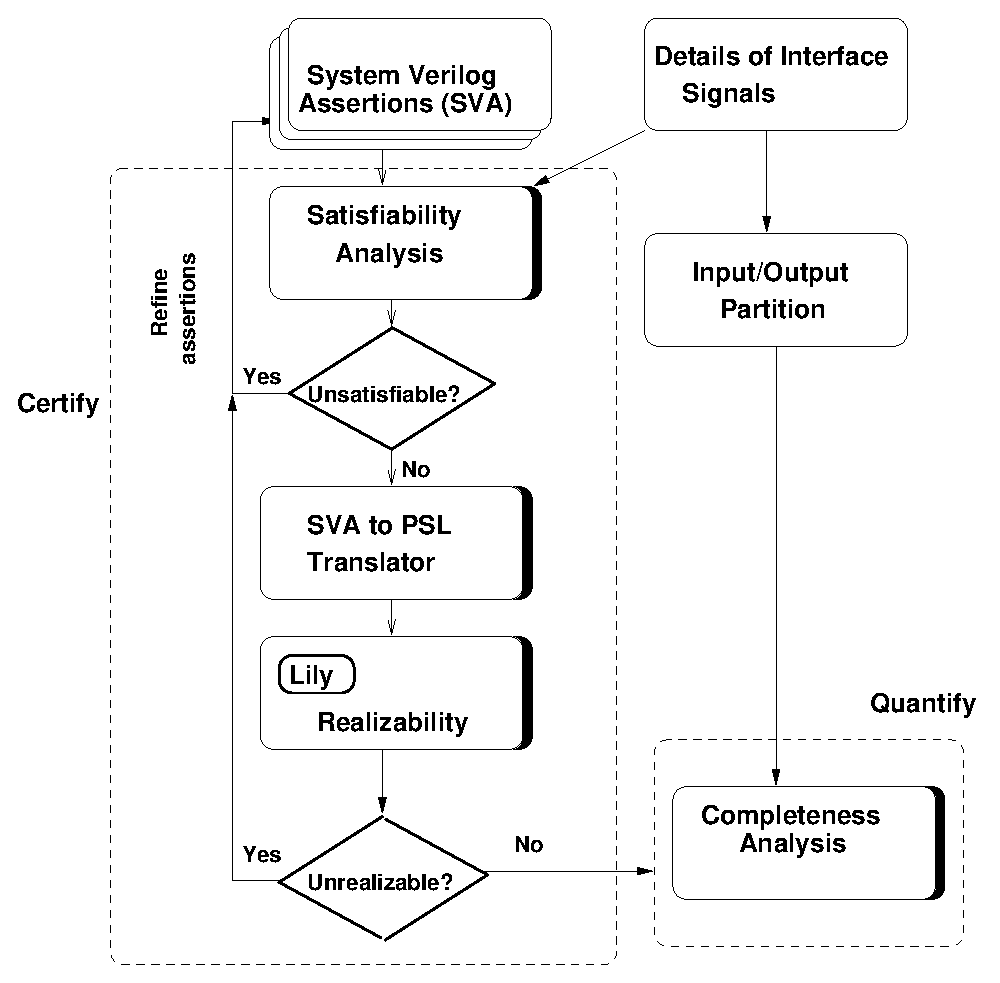
\includegraphics[scale=0.45]{fig0.eps}
\caption{The Architecture of CheckSpec} \label{fig0}
\end{figure}
\noindent
CheckSpec comprises of two main engines:

\begin{itemize}

\item {\bf Certify:} This is used for consistency analysis of SVA assertions. 
	In particular, this takes into account two types of assertion 
	inconsistencies, namely (a) satisfiability violations and 
	(b) implementability or realizability violations. The methods 
	underlying the tool are standard~\cite{roadmap}. Certify has 
	several building 
	blocks. The main components of this engine developed by us are as follows:
\begin{itemize}

\item {\bf A satisfiability checker for SVA} for checking satisfiability 
	of SVA specifications. This supports facilities for both bounded and 
	unbounded satisfiability checking using a symbolic approach.
\item {\bf A realizability checker for SVA} for realizability or 
	implementability analysis of SVA specifications. 
\end{itemize}

\item {\bf Quantify:} This is used for coverage estimate of 
	an assertion suite.  This is independent of any implementation 
	and can be obtained directly from the properties. 
\end{itemize}

\noindent
Fig~\ref{fig0} shows the architecture of our tool. The
tool accepts the assertions in SVA with the information 
of the interface signals (direction, width etc).
On the given set of assertions, we first perform the consistency check 
using Certify. If we have any violation, the specification needs 
to be refined. Once the specification passes the satisfiability check, it is 
subjected to realizability analysis. For this, we have
used Lily~\cite{lily}, a realizability checker for LTL and PSL.
Lily implements the most state-of-the-art algorithms for realizability.
The certified assertions in SVA are translated to PSL using an in-house 
{SVA to PSL translator} and Lily is used for realizability checking. 
Lily has support for a limited subset of PSL 
and hence, our translator also supports the supported subset. 
Once the Certify loop is closed, we perform the 
completeness analysis on the given set of assertions.
This step uses the realizability checker of Certify 
to deduce the coverage. 

The notions of satisfiability and realizability of temporal assertions 
have been well studied in the verification community for 
LTL~\cite{roadmap}. The main novelty of CheckSpec is in 
adopting these problems in the SVA context. Our work on completeness 
analysis is based on the idea proposed in~\cite{das:05} over LTL. Our 
contribution has been to extend this to SVA and provide a prototype 
implementation for analyzing SVA assertion suites. The fundamental idea 
used in~\cite{das:05} is to use a single stuck-at fault model as the 
reference, and verify the realizability of the specification in the presence 
of the fault to determine coverage gaps. If the given specification
becomes unrealizable in the presence of a fault then it should lead to a 
refutation if any design exhibits that fault. Otherwise it is inert to the
fault and the fault is not covered. 

\section{CheckSpec: Major Building Blocks} \label{sec4}
\noindent
{\bf Parser: Lex AND Yacc} 
Lex is an unix utility that parses the input file of characters.It uses 
regular expression matching to tokenize the contents of the file.Rules 
for the tokens are written in the lex file.Maching the patterns of the 
rules lex generate tokens.Each rule specified in the lex has an associated
action.Typically this action returns a token which represents the matced string 
for subsequent use by the parser.The following represents a lex pattern and action:

[0-9]+(\.[0-9]+)? { 
    yylval.value = atof(yytext);
    return NUMBER;
}

yacc: Yet Another Compiler Compiler is an unix utility that parses a stream
of token generated by lex according to the user specified grammer.Our yacc source 
program has three parts :
  
  declarations
  
  %%
    
  translation rules
  
  %%
  
  C routines
  
{\bf Declaration part :}
  Declaration part can have two section.In the first section delimited by 
  %{ and %}. There we included all cpp files and declared global variables.
  %{
  include "eeConstExpr.h"
  include "eeNamedExpr.h"
  
  eeExpr *store;
  %}
    
  In the next section , we defined a union datatype,tokens and assciations.
  %union
  {
    char *str;
    double value;
  }

  %token <str> ID
  %token <str> KWD

  %right LE GE
 
 This two sections are optional.
 
 Declaration Section ends with %%.
 
 {\bf translation rules part :}
 
 In this section the grammars are specified for the parser.Each rule signifies 
 a grammer and associated with a semantic action.
 
 program: program VarDeclStmt | VarDeclStmt | program asStmt | asStmt;
    
 
This sextion also ends with %%.

{\bf C routines :}

C subroutines are called from this section.In our code we have called
yyfinalize() routine.
   
   

\noindent
{\bf ToYicesTranslator:} After parsing we get a symbol table and a syntax tree.
Using this symbol table ToYicesTranslator generates an output file that can run 
on Yices.Our input specification can have declaration statement, Assert statement 
and Assume statement.This statement can be mathematical expression containing infix 
notation and not necessarily all expressions be bianry. But Yices works on postfix 
binary expression.This tool converts any expression into a postfix binary expression.

For example : Let us concider a statement assert (a + b + c = 0);
              To work on yices, this expression should be written as
               
                 (assert( = (+ (+ a b) c) 0))
                 
Symbol Table is basically a datastructure maintained by the compiler to keep information
about the variables. In our tool, the generated symbol table is used to contain variables 
name and their value.

Syntax tree represents an expression in a tree datastructure.Each node of a syntax tree 
is either a terminal or a non-terminal or may be a symbol.
                 
                 
a Syntax tree....



\noindent
{\bf Yices:SMT solver} 

Yices ia a Satisfiability Mopdulo solver to determine the satisfiability of the given assert 
and assume statement. In a yices file the variables are defined, then assert and assume statement
are written on this variables and have .ys extension. 




\begin{figure}[!h]
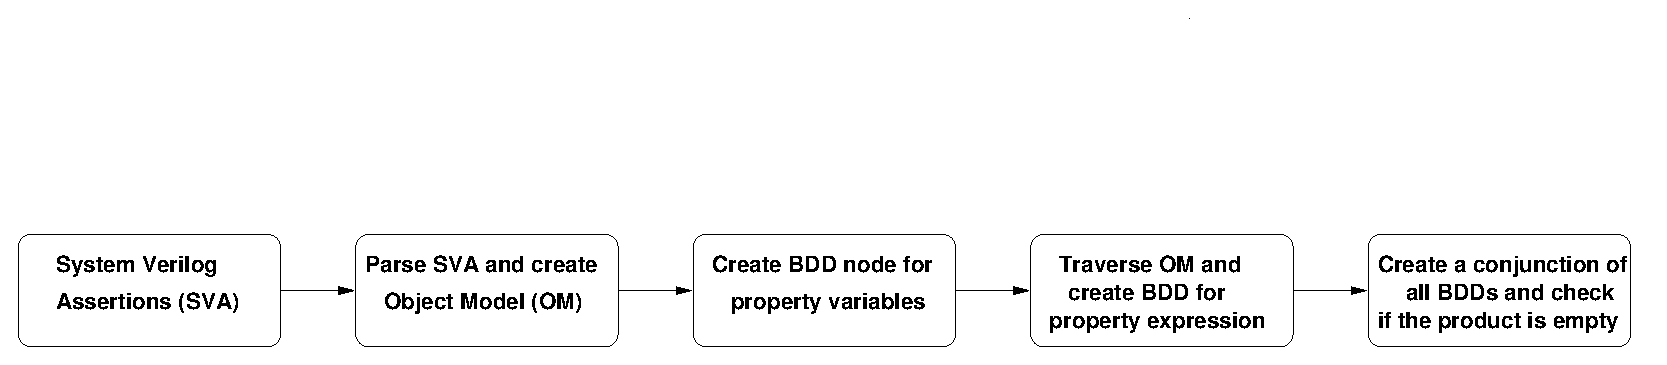
\includegraphics[scale=0.45]{fig1.eps}
\caption{Work-Flow of the satisfiability checking engine} \label{fig1}
\end{figure}

\noindent
{\bf Bounded Satisfiability Engine:} The idea behind this is to 
reduce SVA satisfiability to an instance of Boolean satisfiability. In 
this mode, apart from the SVA specifications, the user is required to give 
as input the depth $k$ (number of clock cycles) for which he wishes to examine 
the satisfiability of the assertions. This depth is utilized to create a 
$k$-bounded Boolean unfolding of each SVA property. The unfolded properties 
are represented using BDDs. The idea behind Boolean unfolding of properties is 
standard~\cite{roadmap} and widely used in the Bounded Model Checking 
(BMC) community. Example~\ref{example3} illustrates this.

\begin{example} \label{example3}
Consider the following SVA properties.
{\tt
\begin{tabbing}
aaaa \= aaa \= aaa \= aaa \= aaa \= aaa \= aaa \= aaa \= aaa \= \kill
\>property P1 \>\>\>\>\>\> \>\>property P2 \\
\>@(posedge clk) a $|->$ \#\#1 b; \>\>\>\>\>\>\>\> @(posedge clk) \#\#1 (a \&\& !b) ;\\
\>endproperty \>\>\>\>\>\>\>\>endproperty
\end{tabbing}
}

\noindent
To illustrate the idea, we create a Boolean unfolding of P1 and P2 with k=2.
{\tt
\begin{tabbing}
aaaa \= aaa \= aaa \= aaa \= aaa \= aaa \= aaa \= aaa \= aaa \= \kill
P1: (a$^1$ |-> b$^2$) $\land$ (a$^2$ |-> b$^3$);
\>\>\>\>\>\>\>P2: (a$^2$ \&\&\ !b$^2$) $\land$ (a$^3$ \&\&\ !b$^3$);
\end{tabbing}
}
\noindent
where $x^t$ represents the value of $x$ in clock cycle $t$. The 
unfolded formulae are individually represented using BDDs.
The conjunction of P1 and P2 gives an empty 
BDD. Hence, we can conclude that they are unsatisfiable. It is 
interesting to note that the bounded satisfiability analysis depends on 
the depth upto which the analysis is done. If k=1, the unsatisfiability 
would not be revealed. 
\end{example}

\noindent
{\bf Unbounded Satisfiability Mode:}
Given a SVA property ${\cal P}$, this approach builds the corresponding 
($tableau$)~\cite{roadmap}. The 
transformation is a straightforward adaptation of the corresponding rules 
for LTL~\cite{roadmap}. Inside Certify, we create a BDD-based 
symbolic representation of the automaton and check for its emptiness as 
per standard methods~\cite{roadmap}. \\

\noindent
{\bf Certify: The Realizability Engine:}
Popular temporal logics such as SVA/PSL do not
syntactically distinguish between inputs and outputs, thereby allowing the
designer to freely mix the input and output signals in the properties. This
leads to realizability problems, since a property that
is consistent when interpreted over a closed system can be inconsistent when
interpreted over all open systems.
A closed system property over a set of variables is {\em satisfiable} if there
exists an assignment of values to the variables in each time step such that
the property is satisfied. On the other hand, the semantics of realizability 
of a property is defined with respect to a open system and its environment.
A property is {\em realizable} if the module is able to set the values of the
output variables in a way that the property is satisfied for {\em all}
possible behaviors of the environment. For example, suppose we have the 
following requirement for an arbiter:
{\em Whenever the high priority req, {\tt hreq}, arrives, the grant
    line, {\tt hgnt}, is given for one cycle with highest priority.}
Suppose we interpret the requirement as -- {\em whenever {\tt hreq} arrives,
assert {\tt hgnt} in the next cycle and lower it after one cycle}. We will
then code this property as:
{\tt
\begin{tabbing}
aaaa \= aaa \= aaa \= aaa \= aaa \= aaa \= aaa \= aaa \= aaa \= \kill
\>\>P0: hreq $|->$ \#\#1 hgnt \#\#1 !hgnt ;
\end{tabbing}
}
\noindent
This property is unrealizable. Suppose {\tt hreq} arrives in two consecutive
cycles, $t$ and $t+1$. We will have a conflict at time $t+2$, because the
request at $t$ will require {\tt hgnt} to be lowered at $t+2$, and the
request at $t+1$ will require {\tt hgnt} to be asserted at $t+2$.

The realizability engine of Certify is a wrapper around Lily that can 
be used for checking realizability of SVA specifications. The flow of 
this has been explained in Figure~\ref{fig0}. Below, we describe its 
major components. \\

\noindent
{\bf SVA to PSL translator:} Given a SVA specification, we translate it 
to its semantically equivalent 
PSL. The transformation rules are one-to-one and intuitively simple for most 
of the SVA constructs. For some SVA features like first\_match, we had to 
generate additional SystemVerilog code to transform it to its semantic 
equivalent. We do not present the details of the transformation rules here. 
For this translator, we utilized our in-house SVA parser to parse the SVA 
specification suite and create the object model (OM). The translation 
is done by a traversal of this OM and decompiling it. \\

\noindent
{\bf Realizability Checking Engine:}
This is a wrapper module that invokes the SVA to PSL translator on a given 
SVA specification suite to generate the equivalent PSL and passes it to 
Lily for realizability checking. 
Lily is a linear logic synthesizer, which can check for realizability of a 
a formal specification. Lily takes a set of 
properties and a partition of the used signals into input and 
output signals and reports if the given set of properties is realizable.
Lily has support for LTL and a limited subset of PSL. \\

\noindent
{\bf Quantify -- Specification Coverage with respect to a fault model:} 
Quantify implements the completeness analysis methods discussed 
in~\cite{das:05}. The core idea behind this approach is as follows: If a 
given specification becomes unrealizable in the presence of a 
fault on an interface signal, it should lead to a
refutation if any design exhibits that fault. Otherwise it is inert to the
fault and the fault is not covered. ~\cite{das:05} uses a single stuck-at 
fault model as the reference. The high-level stuck-at fault model is quite 
effective in practice for finding input and output signals whose behaviors 
have not been appropriately expressed in the assertion specification. 

Quantify reads as input the interface signal 
list (name, width, direction) and the SVA specification suite to be 
analyzed for completeness. The properties are first translated to 
PSL and then the analysis engine is invoked. 
The analysis engine is written using Perl.

\section{Results} \label{sec5}
We tested the algorithms on 2 of our in-house assertion IPs, namely, the ARM
AMBA AHB~\cite{ARM} protocol suite and the OCP~\cite{ocp} protocol suite. 
CheckSpec found some anomalies where properties turned out to be
unsatisfiable. Some properties turned out to be unrealizable when
interpreted over individual modules due to improper decomposition of 
the system level assertions into the module level ones. Certify 
pointed out interesting inconsistencies in the assertion suite.
Quantify was used to deduce the coverage of the properties with respect 
to single stuck-at faults on the signals. 

{\footnotesize
\begin{table*}[!h]
\begin{center}
\begin{tabular}{|c|c|c|c|c|c|c|c|c|c|c|c|c|}
\hline
Ckt  &\#i/p  &\#o/p& \#Ass. & \# B. Sat. & \# U. Sat. &  
Tr. & \#Ass. & \# Rlz. & \% Op. & \% Ip. & Tm \\ \hline
AHB Master & 11 & 9 & 22 & 20.2 & 43.16 & 3.2 & 15 & 2043.16& 85 & 83 & 2067.1\\ \hline 
AHB Slave & 13 & 4 & 9 & 18.33 & 28.3 & 4.7 & 8 & 192.3 & 72 & 95 & 1768.3 \\ \hline
AHB Arbiter & 14 & 3 & 5 & 18.5 & 21 & 3 & 5 & 19.6 & 75 & 75 & 1578.3 \\ \hline
OCP Master & 26 & 25 & 63 & 78.6 & 211.5 & 99.1 & 35 & NT & NT & NT & NT \\ \hline
OCP Slave & 24 & 22 & 34 & 58.5 & 95.3 & 68.1 & 25 & 2219.6 & 78 & 87 & 2578.3 \\ \hline

\end{tabular}
\end{center}
\caption{Results for ARM AMBA AHB and OCP} \label{tab1}
\end{table*}
}

\noindent
Table~\ref{tab1} shows the runtimes on on a 2.4 Ghz Pentium-IV with 1 GB RAM.
Column 1 indicates the interface type (master / slave / arbiter), while 
Columns 2 and 3 show the number of input and output signals in these
interfaces respectively. Column 4 shows the number of assertions.
Columns 5 and 6 show the satisfiability checking time (in 
seconds) using the bounded satisfiability mode and the unbounded mode 
respectively. We used k=10 (chosen arbitrarily) as the analysis depth for 
the bounded satisfiability mode. Column 7 shows the time required to 
translate the SVA assertions to equivalent PSL. Column 8 
shows the number of assertions that could be used for realizability and 
coverage analysis (limited support of Lily) while Column 9 
shows the checking time. Columns 10 and 11 respectively 
show the coverage obtained for the output and input signals while Column 12 
shows the time required for completeness analysis. All times are in seconds. 
For the OCP Master, Lily could not handle the large number of assertions, 
hence the analysis did not terminate (indicated as NT in Table~\ref{tab1}).

{\small
\begin{thebibliography}{99}

\bibitem{ARM} {\em ARM AMBA Specification Rev 2.0}, http://www.arm.com

\bibitem{das:05} Das, S. et al,
    Formal Methods for Analyzing the
    Completeness of an Assertion Suite against a High-Level Fault model,
    In VLSI Design, 2005.

\bibitem{roadmap} Dasgupta, P., A Roadmap for Formal Property Verification,
        Springer 2006.

\bibitem{lily} Lily, http://www.ist.tugraz.at/staff/jobstmann/lily/

\bibitem{ocp} Open Core Protocol, http://www.ocpip.org 

\end{thebibliography}

\end{document}
